%%%%%%%%%%%%%%%%%%%%%%%%%%%%%%%%%%%%%%%%%
% Beamer Presentation
% LaTeX Template
% Version 1.0 (10/11/12)
%
% This template has been downloaded from:
% http://www.LaTeXTemplates.com
%
% License:
% CC BY-NC-SA 3.0 (http://creativecommons.org/licenses/by-nc-sa/3.0/)
%
%%%%%%%%%%%%%%%%%%%%%%%%%%%%%%%%%%%%%%%%%

%----------------------------------------------------------------------------------------
%	PACKAGES AND THEMES
%----------------------------------------------------------------------------------------

\documentclass{beamer}

\mode<presentation> {

% The Beamer class comes with a number of default slide themes
% which change the colors and layouts of slides. Below this is a list
% of all the themes, uncomment each in turn to see what they look like.

%\usetheme{default}
%\usetheme{AnnArbor}
%\usetheme{Antibes}
%\usetheme{Bergen}
%\usetheme{Berkeley}
%\usetheme{Berlin}
%\usetheme{Boadilla}
%\usetheme{CambridgeUS} %Color rojo, me gusta
%\usetheme{Copenhagen} %Ta bueno
\usetheme{Darmstadt} % Este es el 1er candidato
%\usetheme{Dresden} % Es lindo y parecido al de arriba
%\usetheme{Frankfurt}
%\usetheme{Goettingen}
%\usetheme{Hannover}
%\usetheme{Ilmenau}
%\usetheme{JuanLesPins}
%\usetheme{Luebeck}
%\usetheme{Madrid}
%\usetheme{Malmoe}
%\usetheme{Marburg}
%\usetheme{Montpellier}
%\usetheme{PaloAlto}
%\usetheme{Pittsburgh}
%\usetheme{Rochester}
%\usetheme{Singapore}
%\usetheme{Szeged}
%\usetheme{Warsaw}

% As well as themes, the Beamer class has a number of color themes
% for any slide theme. Uncomment each of these in turn to see how it
% changes the colors of your current slide theme.

%\usecolortheme{albatross}
%\usecolortheme{beaver}
%\usecolortheme{beetle}
%\usecolortheme{crane}
%\usecolortheme{dolphin}
%\usecolortheme{dove}
%\usecolortheme{fly}
%\usecolortheme{lily}
%\usecolortheme{orchid}
%\usecolortheme{rose}
%\usecolortheme{seagull}
%\usecolortheme{seahorse}
%\usecolortheme{whale}
%\usecolortheme{wolverine}

%\setbeamertemplate{footline} % To remove the footer line in all slides uncomment this line
%\setbeamertemplate{footline}[page number] % To replace the footer line in all slides with a simple slide count uncomment this line

%\setbeamertemplate{navigation symbols}{} % To remove the navigation symbols from the bottom of all slides uncomment this line
}

\usepackage{graphicx} % Allows including images
\usepackage{booktabs} % Allows the use of \toprule, \midrule and \bottomrule in tables
\usepackage{listings}
%\usepackage{url}
\usepackage{hyperref}
\usepackage[spanish]{babel}
\usepackage[utf8]{inputenc}
%----------------------------------------------------------------------------------------
%	TITLE PAGE
%----------------------------------------------------------------------------------------

\title[Flujo Digital]{Instalación y Configuración de un Flujo de Diseño Digital} % The short title appears at the bottom of every slide, the full title is only on the title page

\author{Leandro Marsó} % Your name
\institute[] % Your institution as it will appear on the bottom of every slide, may be shorthand to save space
{
Córdoba\\ % Your institution for the title page
\medskip
\textit{elleandro@gmail.com} % Your email address
}
\date{\today} % Date, can be changed to a custom date

\begin{document}


\lstset{
basicstyle=\ttfamily,                   % Code font, Examples: \footnotesize, \ttfamily
frame=none,                             % A frame around the code
tabsize=2,                              % Default tab size
captionpos=b,                           % Caption-position = bottom
breaklines=false,                        % Automatic line breaking?
breakatwhitespace=false,                % Automatic breaks only at whitespace?
showspaces=false,                       % Dont make spaces visible
showtabs=false,                         % Dont make tabls visible
showstringspaces=false,
commentstyle=\color{red},
keywordstyle=\color{blue},
}


\begin{frame}
\titlepage % Print the title page as the first slide
\end{frame}

\begin{frame}
\frametitle{Contenido} % Table of contents slide, comment this block out to remove it
\tableofcontents % Throughout your presentation, if you choose to use \section{} and \subsection{} commands, these will automatically be printed on this slide as an overview of your presentation
\end{frame}

%----------------------------------------------------------------------------------------
%	PRESENTATION SLIDES
%----------------------------------------------------------------------------------------
\begin{frame}
\frametitle{DEF/LEF}

\textbf{DEF}: Desing Exchange Format \\
\textbf{LEF}: Library Exchange Format \\


El formato es el mismo para ambos, pero cuando se utiliza para describir un bloque, se llama DEF, y para una libreria de celdas estandars se denomina LEF.
Se puede encontrar un archivo .lef con las reglas y definiciones de la tecnolog\'ia, y otro .lef con la librer\'ia de celdas est\'andar.\\
Este formato es lo que usa el ruteador y el placer (entre otras herramientas) para conocer aspectos fisicos de las celdas y los bloques. Tiene informaci\'on del layout y de la tecnolog\'ia. 



\end{frame}

%------------------------------------------------
\begin{frame}
  \begin{figure}[ht]
      \centering
      \scalebox{.65}{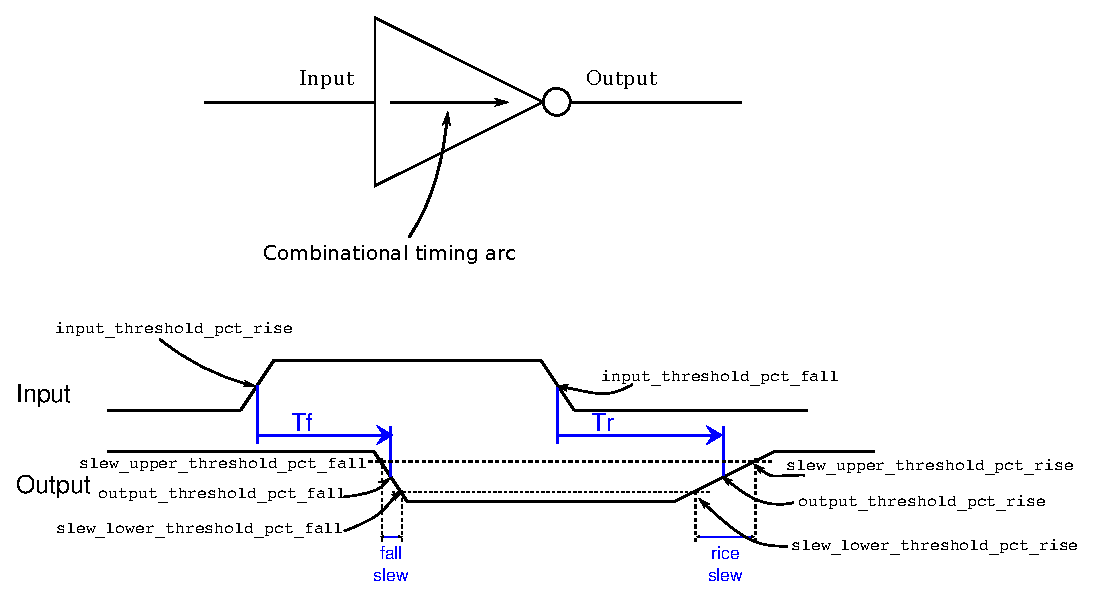
\includegraphics[angle=0]{figuras/inout-timing.eps}}
    \end{figure}
  
\end{frame}

%------------------------------------------------
\begin{frame}
  \begin{figure}[ht]
      \centering
      \scalebox{.65}{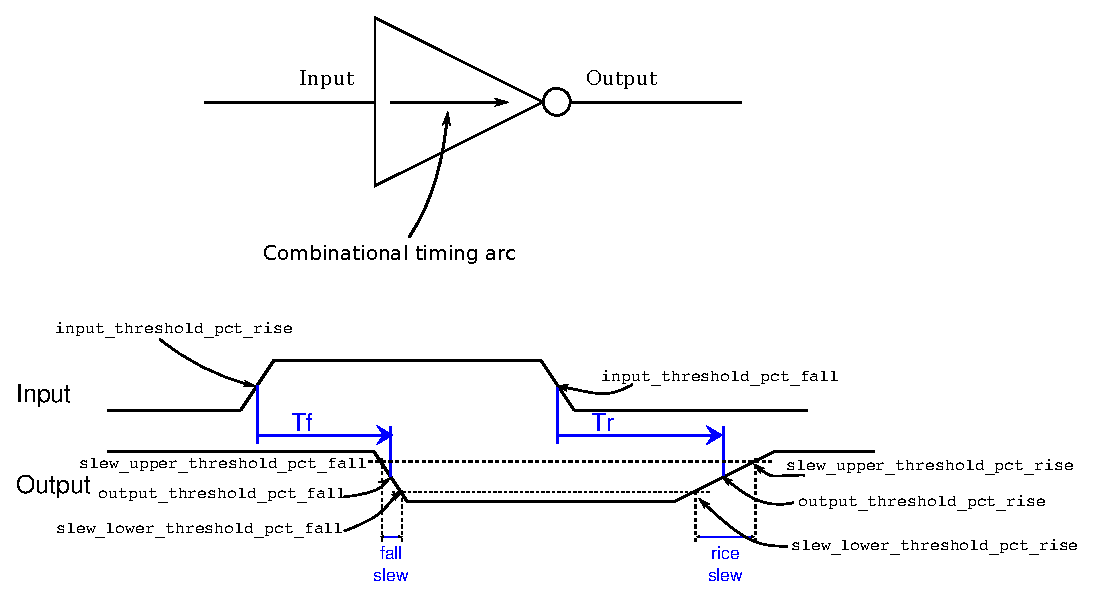
\includegraphics[angle=0]{figuras/inout-timing.eps}}
    \end{figure}
  
\end{frame}

%----------------------------------------------------------------------------------------

\begin{frame}
\textbf{NLDM: Non-Linear Delay Model} 
   \begin{figure}[ht]
      \centering
      \scalebox{.30}{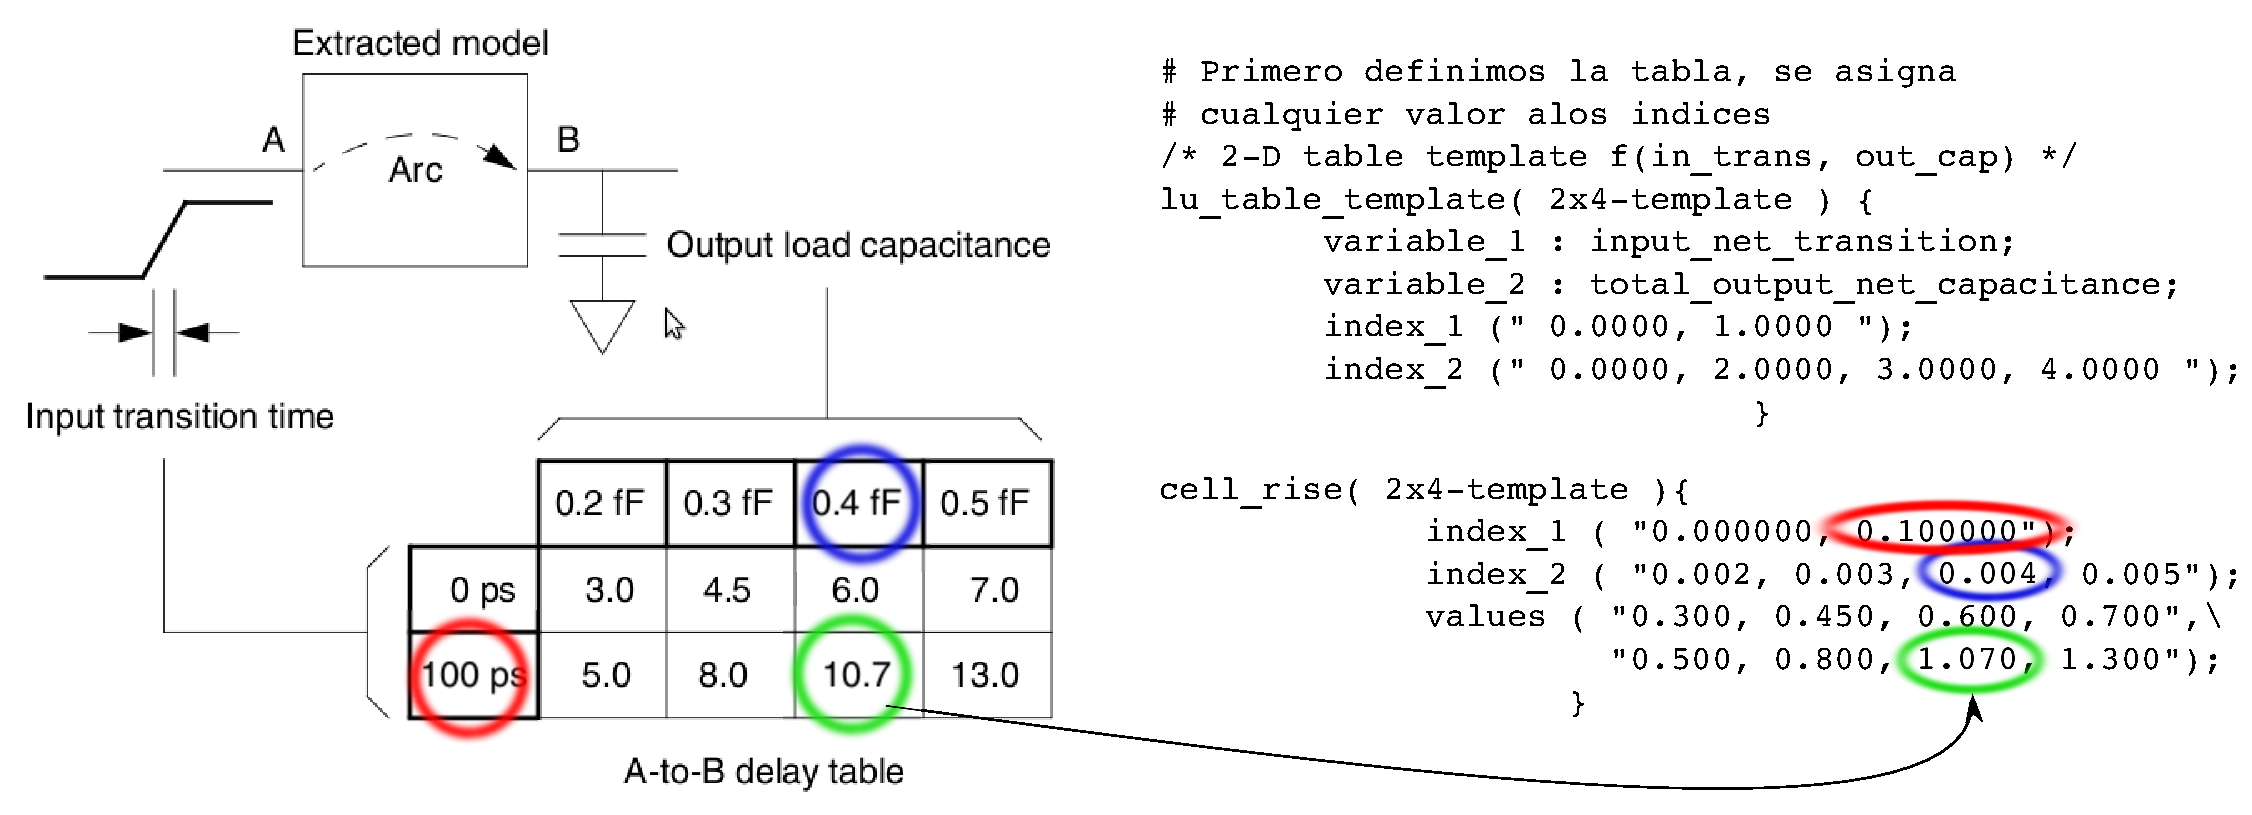
\includegraphics[angle=0]{figuras/delay-table.eps}}
    \end{figure}
\end{frame}


%----------------------------------------------------------------------------------------
\begin{frame}
\frametitle{DEF/LEF}
DEF: Desing Exchange Format \\
LEF: Library Exchange Format \\

\begin{center}¿Qué datos nos brinda este formato?
\end{center}
    \begin{itemize}
    \item Informaci\'on sobre DRC \'util para el ruteador, por ejemplo la separación mínima entre cables, m\'aximo ancho de pista, capas de obstrucción, Antenna Rules.
    \item B\'asicamente es informaci\'on de layout mas alguna informaci\'on extra \'util para el ruteador. Orientaci\'on de la celda o macrocelda.  
    \end{itemize}
\end{frame}

%------------------------------------------------
\begin{frame}
  \frametitle{Modelos de timing y potencia} 

\textbf{NLDM: Non-Linear Delay Model} 

Es una forma de expresar los Delay, Timing Checks y Output Slew (tiempo de transici\'on) de bloques. Asume carga capacitiva pura, utilizando capacidad equivalente en el caso de que la resistencia no es despreciable. 
 
\end{frame}

%----------------------------------------------------
\begin{frame}
  \frametitle{Modelos de timing y potencia} 

 \textbf{NLDM: Non-Linear Delay Model} 
   \begin{figure}[ht]
      \centering
      \scalebox{.30}{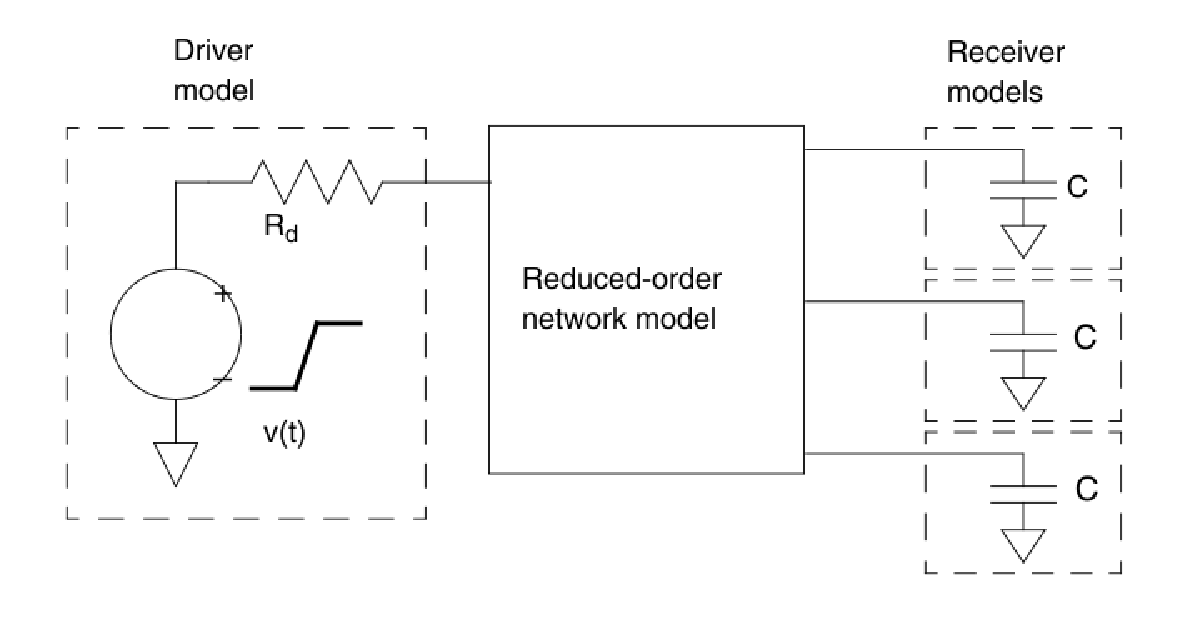
\includegraphics[angle=0]{figuras/nldm-model.eps}}
    \end{figure}
    Se especifica los tiempos según una tabla de 2 entradas:
    \begin{itemize}
	\item El tiempo de transición de la fuente de tensión a la entrada (driver)
	\item Capacidad de carga a la salida (receptor)
\end{itemize}

\end{frame}
%----------------------------------------------------


\begin{frame}
\Huge{\centerline{Fin}}
\end{frame}

%----------------------------------------------------------------------------------------

\end{document} 
